\documentclass[a4paper,11pt]{article}
% Use ctrl + alt + V to view live pdf

% Packages
\usepackage[utf8]{inputenc} % For encoding
\usepackage[T1]{fontenc} % Better handling of accented characters and hyphenation
\usepackage{microtype} % Improves spacing and justification
\usepackage{amsmath, amssymb} % For equations and symbols
\usepackage{graphicx} % For including graphics/images
\usepackage{caption} % For customizing figure and table captions
\usepackage{subcaption} % For subfigures and subcaptions
\usepackage{float} % For fixing figure and table positions
\usepackage{booktabs} % For professional-looking tables
\usepackage{siunitx} % For consistent typesetting of units and numbers
\usepackage[margin=2cm]{geometry} % Adjusts page margins
\usepackage{fancyhdr} % For custom headers and footers
\usepackage{lmodern} % For a professional-looking font (main body font)
\usepackage{titlesec} % For title customization
\usepackage{array} % For custom table formatting
\usepackage[colorlinks=true, linkcolor=black, citecolor=blue, urlcolor=blue]{hyperref} % Colored links without boxes
\usepackage{cleveref} % For improved cross-referencing    
\usepackage{multirow}
\usepackage{enumitem}
\usepackage{listings}
\usepackage{xcolor}
\usepackage{textcomp}
\usepackage{tabularx}
\usepackage{changepage}
\usepackage{tikz}
\usepackage{pdfpages}
\usepackage[table]{xcolor}
\usepackage{tocloft}
\usepackage{multicol}
\renewcommand{\lstlistingname}{Program}

\titleformat{\section}{\Large\bfseries}{\thesection}{1em}{}
\titleformat{\subsection}{\large\bfseries}{\thesubsection}{1em}{}

\pagestyle{fancy}
\fancyhf{}
\fancyhead[L]{\textit{Smart Plant Watering System}}
\fancyhead[R]{\textit{Will Hewes | wh365@cam.ac.uk}}                        
\setlength{\headheight}{10pt}                         

\begin{document}
\begin{center}
    {\Huge \textbf{Smart Plant Watering System}}\\[0.5em]
    \textbf{Marketing Data Sheet}
\end{center}
\vspace{-1.5em}

\titleformat{\section}[block]{\Large\bfseries\filcenter}{}{1em}{}
\titleformat{\subsection}[block]{\large\bfseries\filcenter}{}{1em}{}

\section*{Overview}
This smart plant watering system offers a cost-effective, 
modular solution for automating plant care. 
Designed around an Arduino Uno and a Python GUI, 
the system autonomously monitors soil moisture and temperature and 
triggers watering via a 3D-printed pinch valve. 
It supports manual or automatic control, visual and sound based warnings, 
and real-time data logging, making it suitable for 
hobbyists, students, or small-scale growers. 
The simple hardware and open-source software architecture ensure easy setup, 
low maintenance, and future expandability.

\vspace{1em}
\begin{center}
    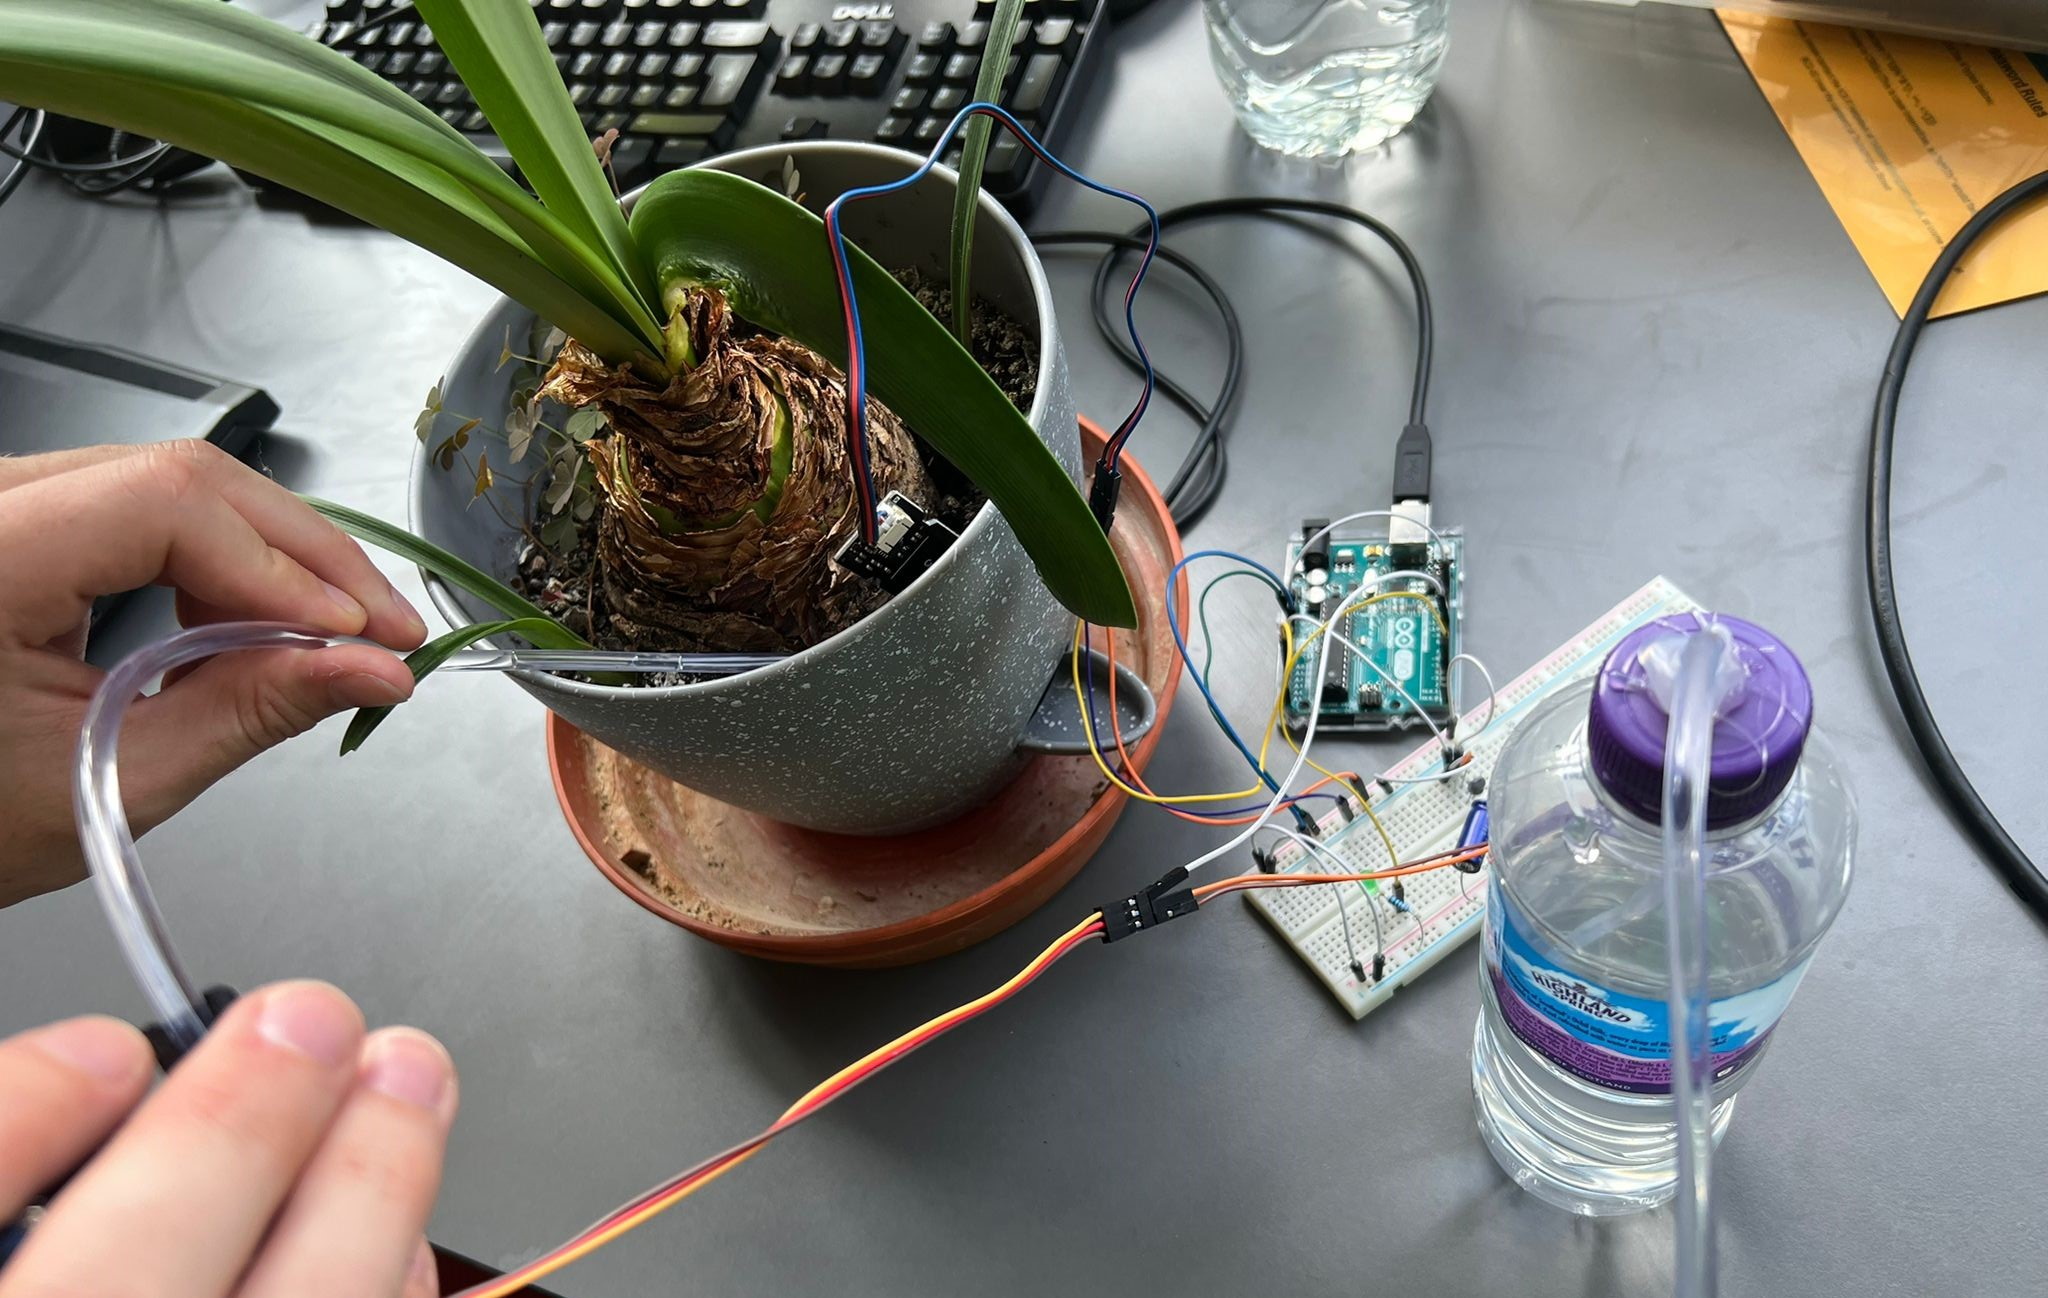
\includegraphics[width=0.9\textwidth]{Images/Setup.jpg}
\end{center}

\vspace{1em}

\section*{Key Features}
\begin{itemize}[leftmargin=1.5em]
    \item \textbf{Real-Time Data Plotting:} 
    Live visualisation of soil moisture and temperature.
    \item \textbf{Robust Serial Communication:} 
    Reliable USB link using PySerial with timeout safeguards.
    \item \textbf{Expandable Hardware:} 
    PCB layout includes reserved ports for additional sensors.
    \item \textbf{Custom 3D-Printed Valve:} 
    Servo-actuated pinch valve designed to fit standard PVC tubing.
    \item \textbf{Safe Actuation Logic:} 
    Safety measures put into place to prevent software faults.
    \item \textbf{Easy Threshold Setting:}
    The system has been designed to make it as easy as possible 
    to set threshold moisture values and environment warning levels,
    guaranteeing the health and safety of your plants.
\end{itemize}

\section*{Why Choose This System?}
\begin{itemize}[leftmargin=1.5em]
    \item \textbf{Affordable:} 
    Total cost of under £12, with cheap expandability available.
    \item \textbf{Unattended Operation:} Designed for extended use with 
    minimal maintenance, ideal for holidays.
    \item \textbf{User-Friendly:} Easy threshold adjustment and 
    one-click manual watering via intuitive GUI.
\end{itemize}

\vspace{1em}

\begin{center}
    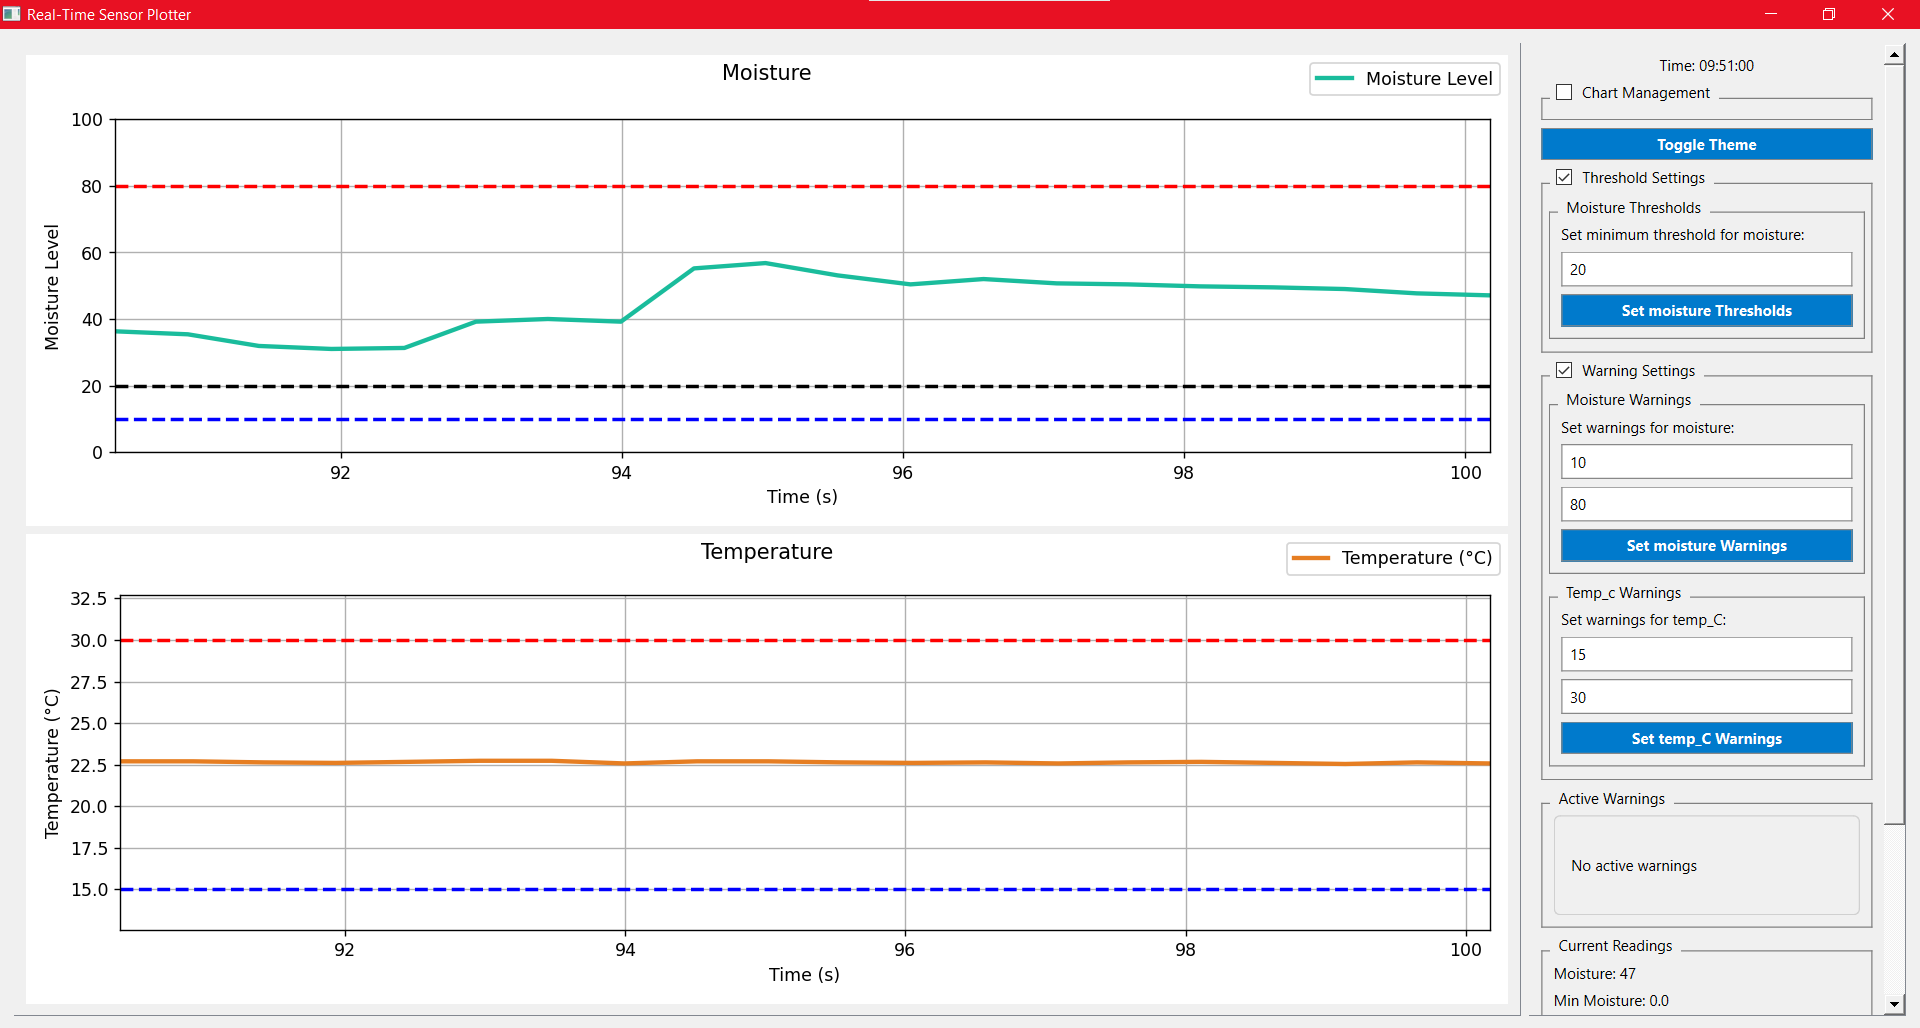
\includegraphics[width=0.9\textwidth]{Images/3 - Threshold Setting.png}
\end{center}

\section*{Specifications}
\vspace{-01em}
\begin{table}[H]
    \centering
    \begin{tabularx}{0.8\textwidth}{>{\bfseries}l X}
        Microcontroller & Arduino Uno R3 \\
        Power Supply & 5V USB or power bank \\
        Soil Sensor & Capacitive moisture sensor \\
        Temperature Sensor & TMP36 + 100 pF capacitor \\
        Valve & Servo-powered 3D-printed pinch valve \\
        Warning Features & Flashing LED, sound alert  \\
    \end{tabularx}
    \label{tab:system_overview}
\end{table}

\section*{Future Improvements}
We are excited to announce there will be more features implemented 
on future systems!

\begin{itemize}[leftmargin=1.5em, nosep]
    \item \textbf{Sensor Expansion:} 
    Humidity and light sensors 
    to provide a more complete environmental profile.
    \item \textbf{Wireless Connectivity:} Bluetooth and Wi-Fi modules for 
    remote monitoring and notifications.
    \item \textbf{Logging:} Extend data logging capabilities 
    for tracking environmental trends over time.
    \item \textbf{Improved GUI Features:} Support multiple tabs and chart types, 
    and enable exporting of plotted data directly from the interface.
    \item \textbf{Water Supply Safeguards:} 
    Add a float switch to monitor the reservoir and prevent dry actuation.
\end{itemize}


\section*{Contact \& Collaboration}
For educational use, licensing inquiries, or industrial integration:\\

\noindent
\textbf{Will Hewes} \\
\texttt{wh365@cam.ac.uk} \\
\textit{University of Cambridge, Department of Engineering}

\end{document}